\section{Análise dos resultados}
Nas seções seguintes iremos comparar resultados obtidos ao executar as estratégias HOM e Mutação Seletiva a cada problemas estudado e em seguida o \textit{score} de cada problema por estratégia.

\subsection{Análise por problemas}
Primeiro iremos mostrar o desempenho de cada uma das estratégias em cada um dos seis problemas estudados.

\subsubsection{Bisect}
\begin{figure}[H]
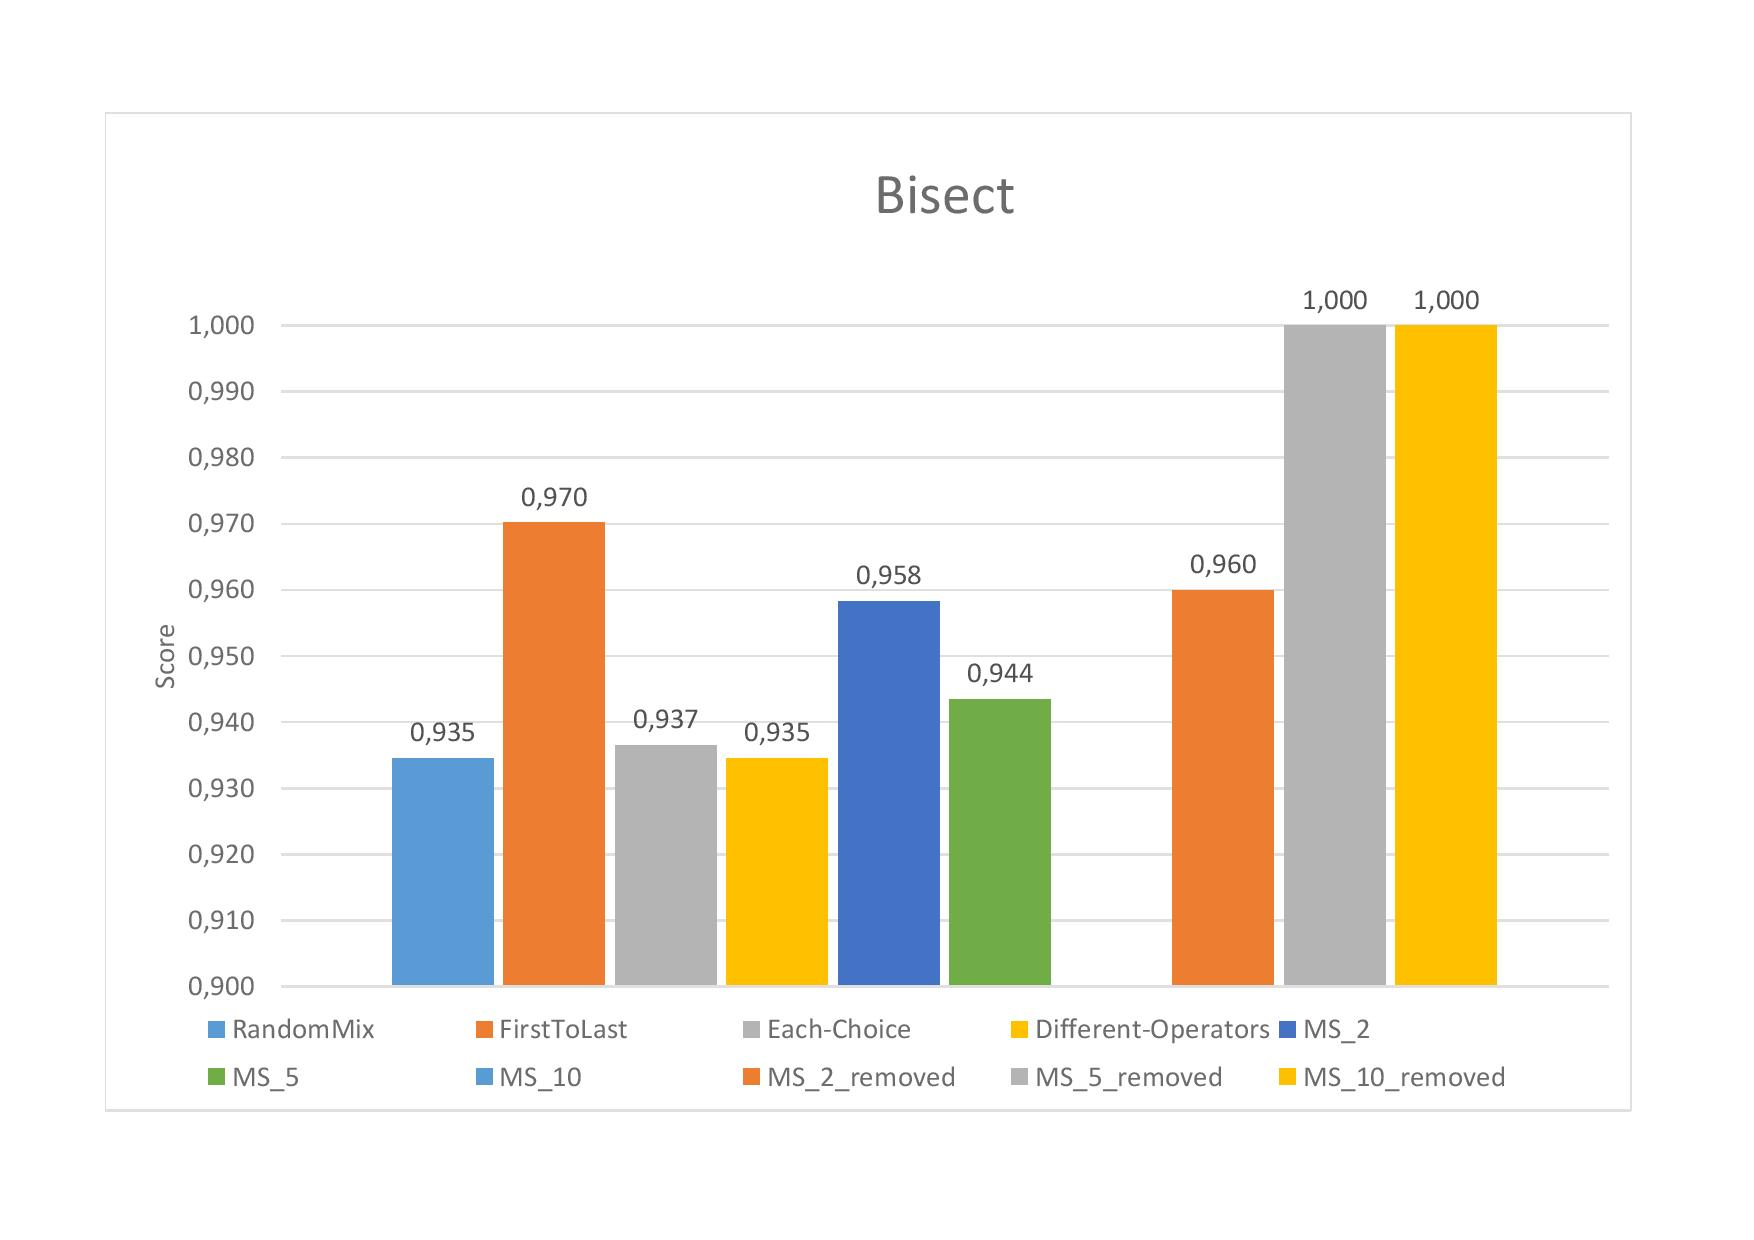
\includegraphics[width=1\textwidth]{graficos/problems/bisect.jpg}
\caption{\textit{Scores} das estratégias no problema Bisect}
\label{fig:bisect}
\end{figure}
No \textit{Bisect} podemos notar que com excessão da MS\_10, as estratégias MS\_2, MS\_5 e MS\_2\_removed se saíram melhores do que 3 dos 4 SOMs. O MS\_2 e seu complemento ganharam com vantagem expressiva aos 3 SOMs.
A estratégia MS\_10 não obteve resultado, isso aconteceu porque a matriz de FOMs fonte possuía mutantes de 10 ou menos operadores, restando nenhum mutante para ser avaliado.

\subsubsection{Bub}
\begin{figure}[H]
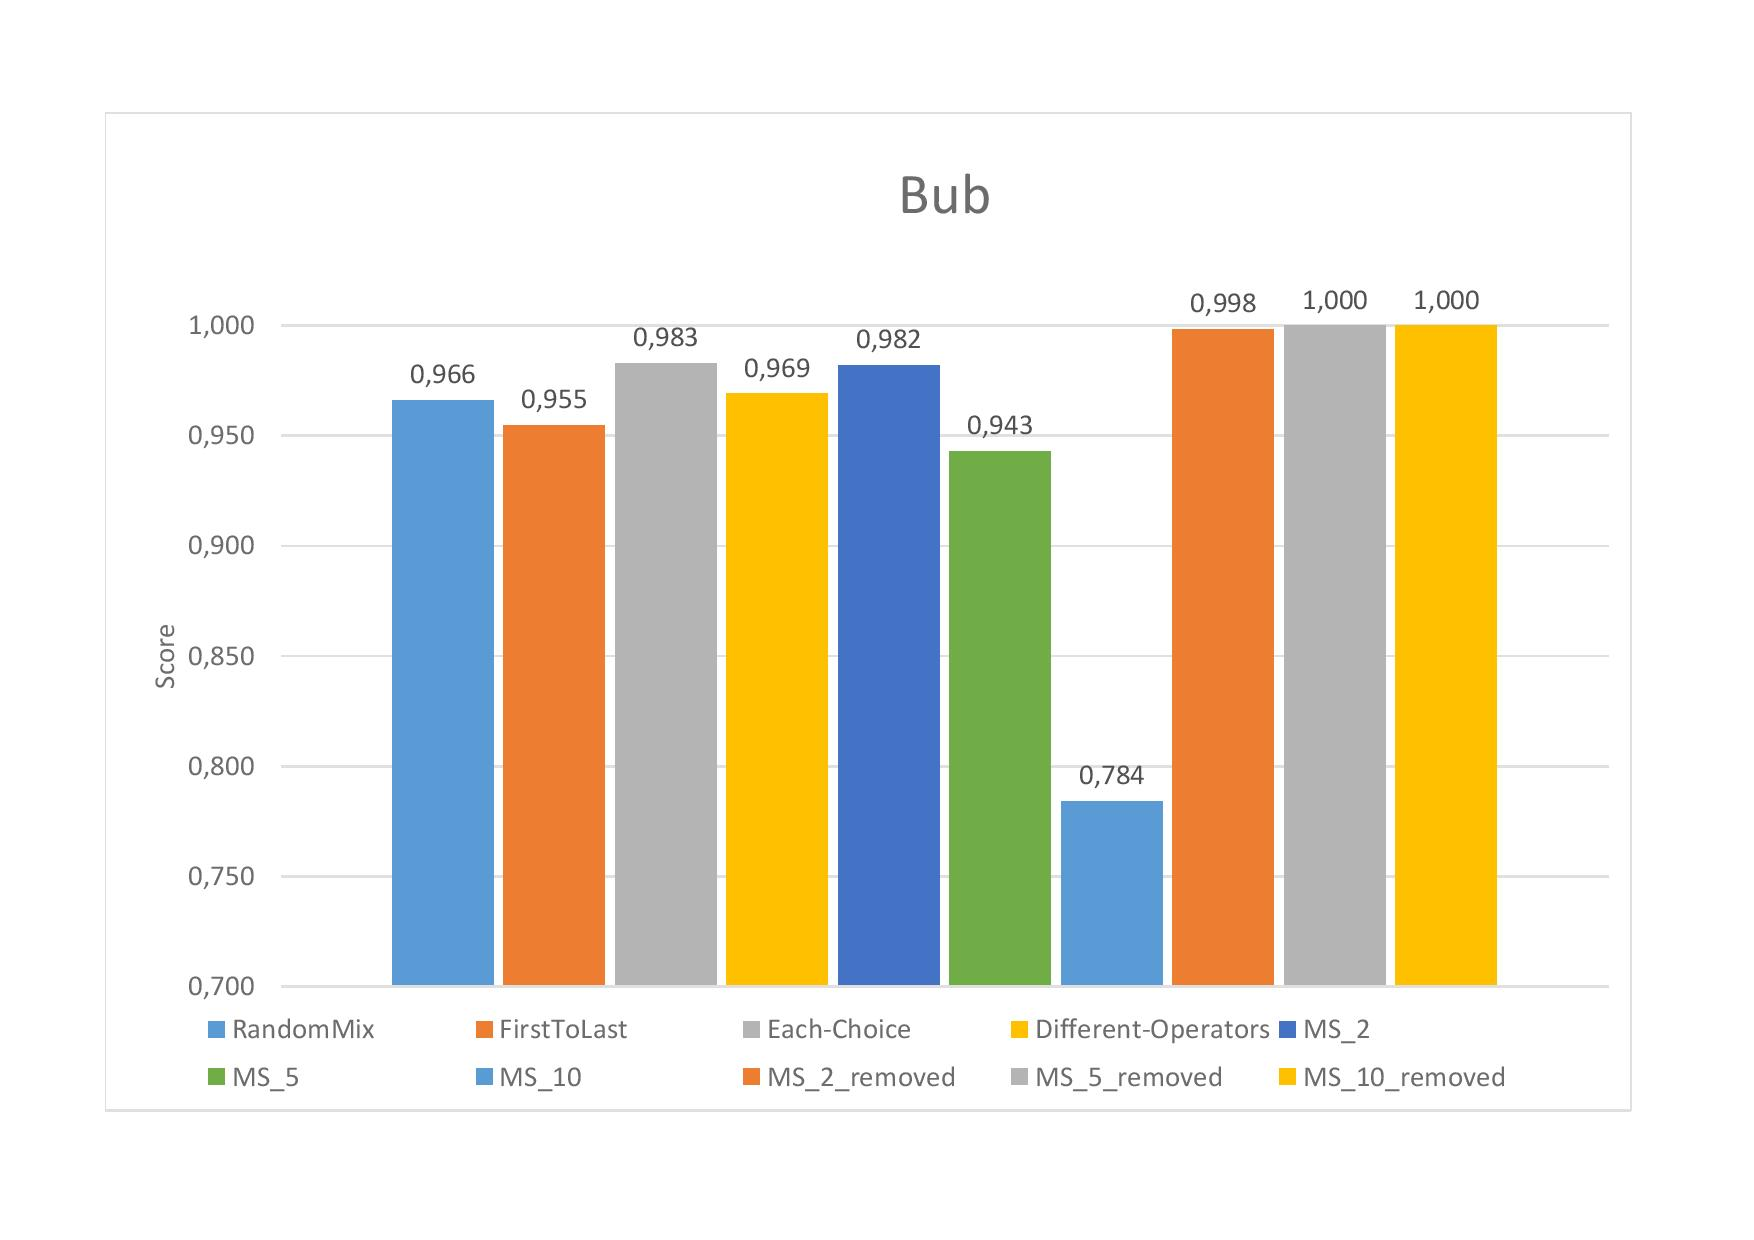
\includegraphics[width=1\textwidth]{graficos/problems/bub.jpg}
\caption{\textit{Scores} das estratégias no problema Bub}
\label{fig:bub}
\end{figure}
No \textit{Bub} podemos notar que novamente o MS\_10 mostrou um desempenho muito abaixo da dos demais e que o MS\_2 praticamente empatou com o SOM que obteve o melhor \textit{score}. Algo a se notar nesse problema, é que os complementos ficaram quase em 1.0, e o MS\_2\_removed, por possui um número menor de mutantes que os demais complementos, começa parecer uma estratégia interessante de se trabalhar.

\subsubsection{Find}
\begin{figure}[H]
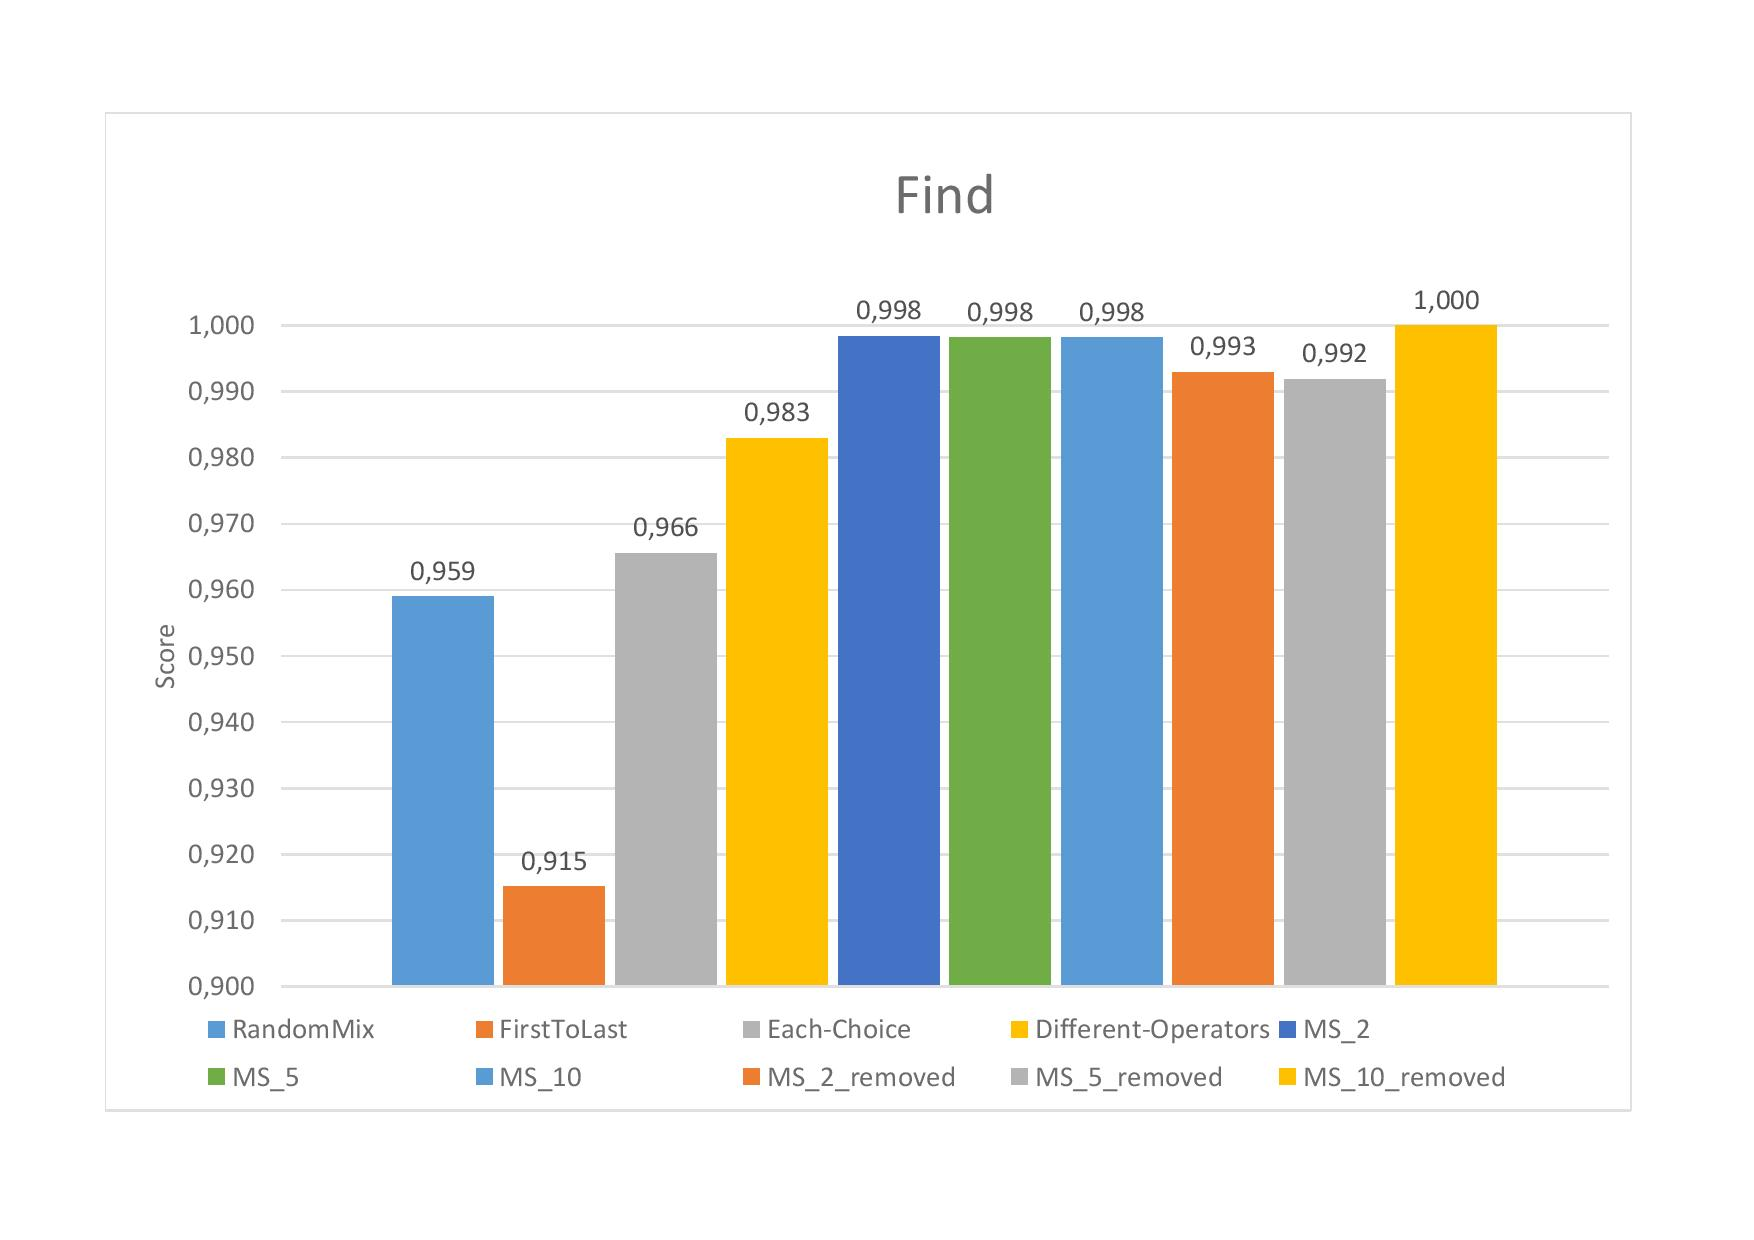
\includegraphics[width=1\textwidth]{graficos/problems/find.jpg}
\caption{\textit{Scores} das estratégias no problema Find}
\label{fig:find}
\end{figure}
Neste problema, todas as estratégias de mutação seletiva se mostraram mais eficazes que os SOMs. Vale lembrar que a estratégia MS\_10 tem um número muito reduzido de FOMs e que a  MS\_2 possui ainda menos, no entanto seus \textit{scores} ainda ficaram próximos ao \textit{score} ideal.

\subsubsection{Fourballs}
\begin{figure}[H]
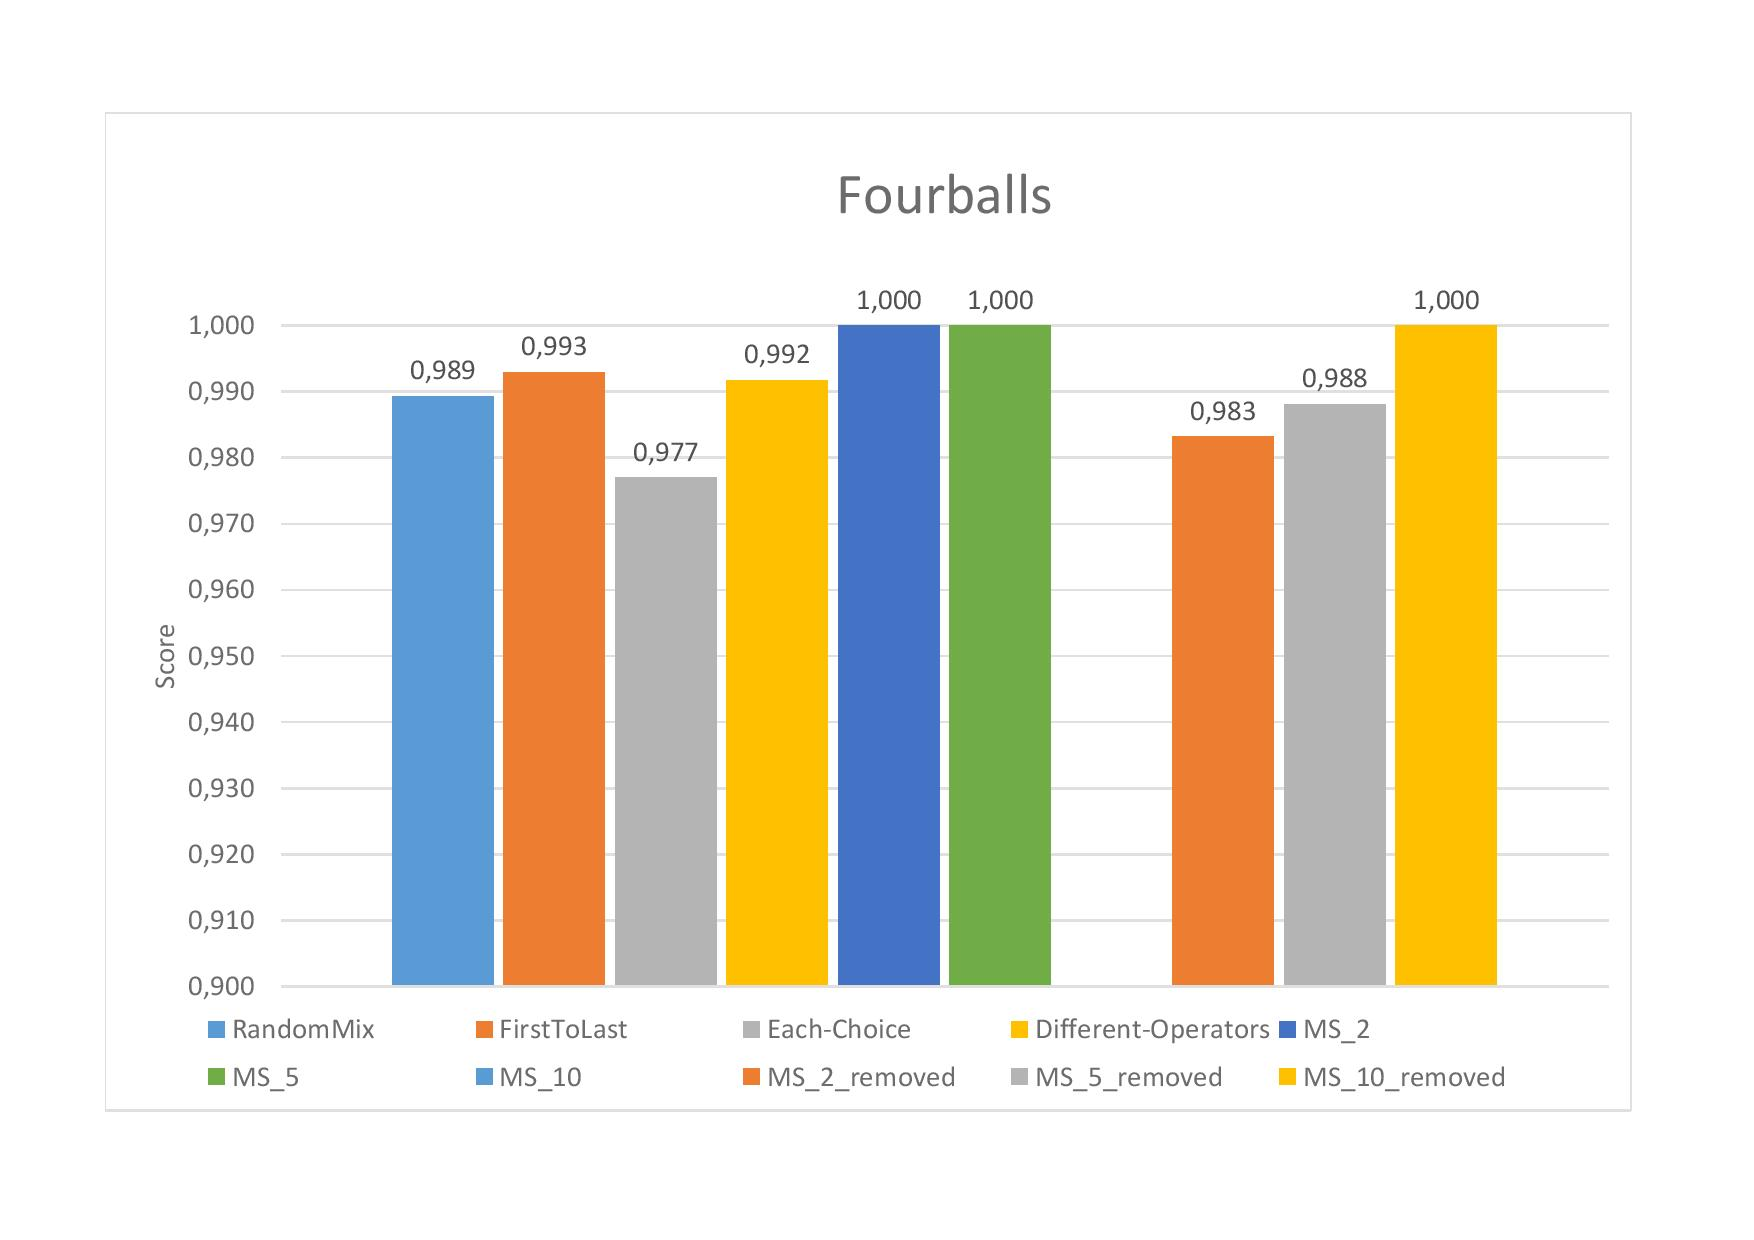
\includegraphics[width=1\textwidth]{graficos/problems/fourballs.jpg}
\caption{\textit{Scores} das estratégias no problema Fourballs}
\label{fig:fourballs}
\end{figure}
No \textit{Fourballs} tanto o MS\_2 quanto MS\_5 obtiveram \textit{score} máximo e seus complementos ficaram próximos dos SOMs estudados, porém como nesse caso temos poucos operadores, a estratégia de mutação seletiva que terá o menor conjunto de mutantes é a MS\_2. 
Novamente a estratégia MS\_10 não obteve resultado porque a matriz de FOMs fonte possuía mutantes de 10 ou menos operadores, restando nenhum mutante para ser avaliado.

\subsubsection{Mid}
\begin{figure}[H]
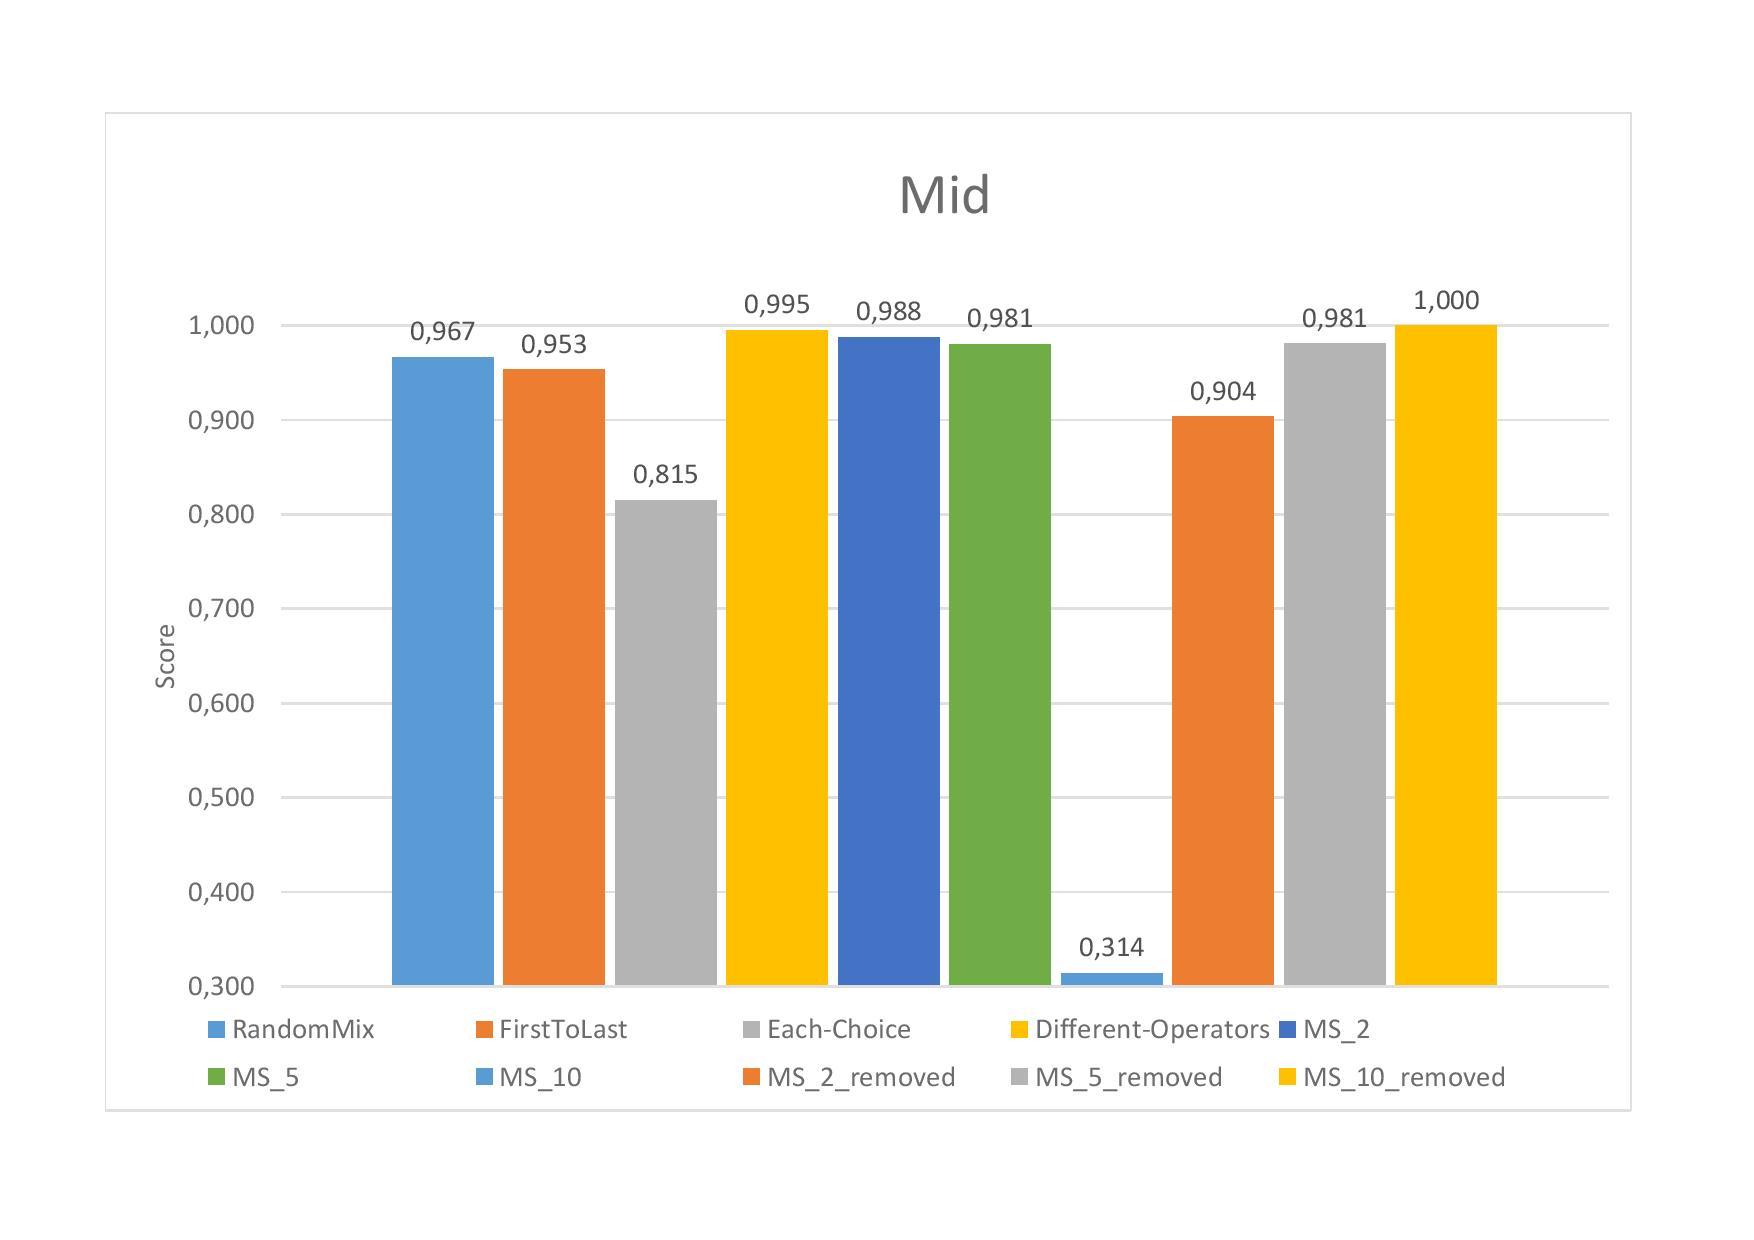
\includegraphics[width=1\textwidth]{graficos/problems/mid.jpg}
\caption{\textit{Scores} das estratégias no problema Mid}
\label{fig:mid}
\end{figure}
A execução para este problema mostra novamente que a estratégia MS\_10 possui um score muito abaixo do ideal, e que as estratégias MS\_2 e MS\_5 novamente se mostraram muito eficientes, perdendo por apenas aproximadamente 0,007 para o SOM \textit{Different-Operators}.
\subsubsection{Triangulo}
\begin{figure}[H]
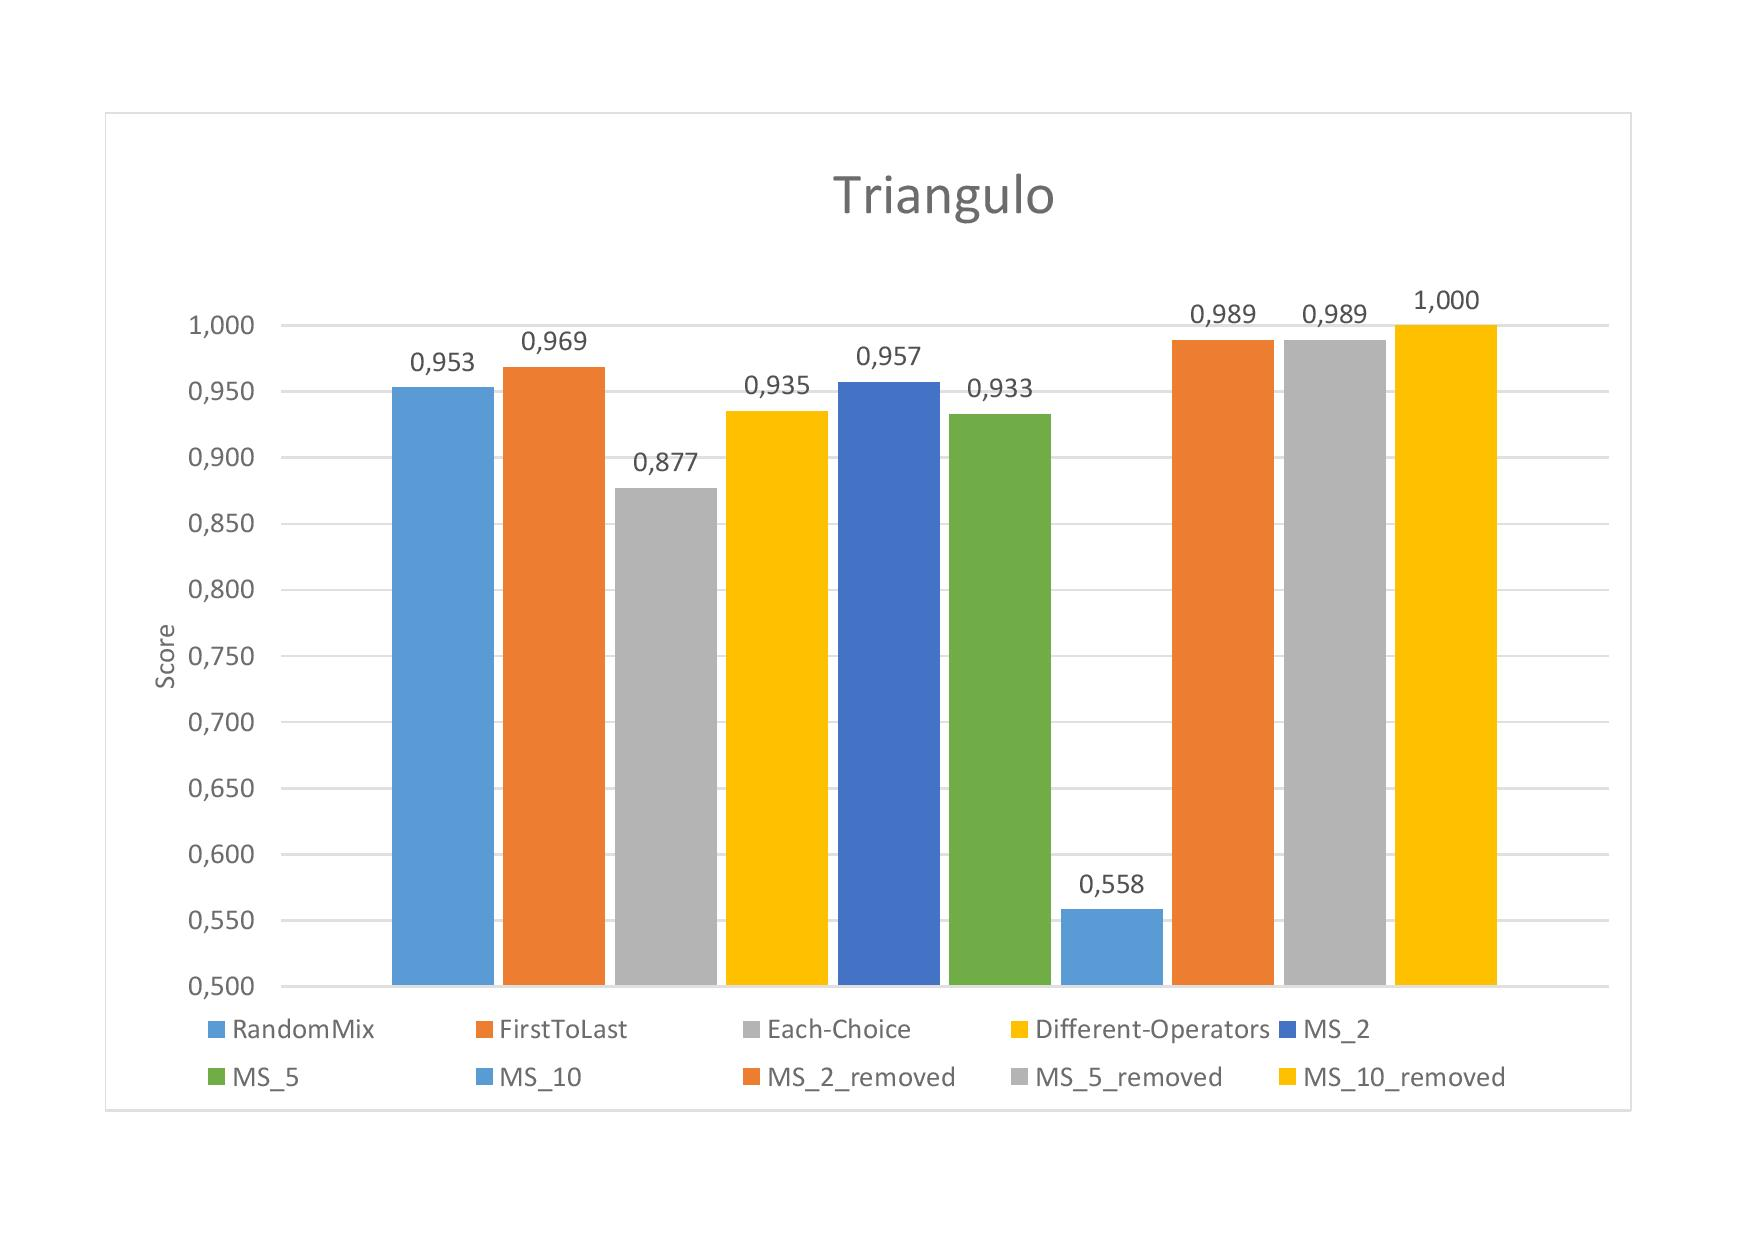
\includegraphics[width=1\textwidth]{graficos/problems/triangulo.jpg}
\caption{\textit{Scores} das estratégias no problema Triangulo}
\label{fig:triangulo}
\end{figure}
Assim como no problema anterior, neste a estratégia MS\_10 se mostra impraticável, enquanto as MS\_2 e MS\_5 mostram um desempenho muito próximo aos outros SOMs com melhores resultados. A MS\_2 teve desempenho inferior a somente a SOM First2Last. Algo interessante neste problema é o desempenho dos complementos de MS\_2 e MS\_5 com \textit{scores} próximos a 1.0.

\subsection{Análise por estratégia}
Nesta seção veremos o score em cada um dos problemas para cada estratégia escolhida assim como iremos fazer algumas comparações com base em alguns dados estatísticos disponíveis na tabela [\ref{tab:stats}] abaixo.
\begin{table}[ht]
\centering
\caption{Dados estatísticos sobre os \textit{scores} de cada estratégia em cada problema}
\label{tab:stats}
\begin{tabular}{|l|l|l|l|l|l|}
\hline
                             & \textbf{Mínimo} & \textbf{Máximo} & \textbf{Máximo-Mínimo} & \textbf{Média} & \textbf{Desvio padrão} \\ \hline
\textbf{RandomMix}           & 0.935           & 0.989           & 0.055                  & 0.961          & 0.016                  \\ \hline
\textbf{FirstToLast}         & 0.915           & 0.993           & 0.078                  & 0.959          & 0.024                  \\ \hline
\textbf{Each-Choice}         & 0.815           & 0.983           & 0.168                  & 0.926          & 0.061                  \\ \hline
\textbf{Different-Operators} & 0.935           & 0.995           & 0.061                  & 0.968          & 0.025                  \\ \hline
\textbf{MS\_2}               & 0.957           & 1.000           & 0.043                  & 0.981          & 0.017                  \\ \hline
\textbf{MS\_5}               & 0.933           & 1.000           & 0.067                  & 0.966          & 0.027                  \\ \hline
\textbf{MS\_10}              & 0.314           & 0.998           & 0.684                  & 0.664          & 0.255                  \\ \hline
\textbf{MS\_2\_removed}      & 0.904           & 0.998           & 0.095                  & 0.971          & 0.033                  \\ \hline
\textbf{MS\_5\_removed}      & 0.981           & 1.000           & 0.019                  & 0.992          & 0.007                  \\ \hline
\textbf{MS\_10\_removed}     & 1.000           & 1.000           & 0.000                  & 1.000          & 0.000                  \\ \hline
\end{tabular}
\end{table}

\subsubsection{Random}
\begin{figure}[H]
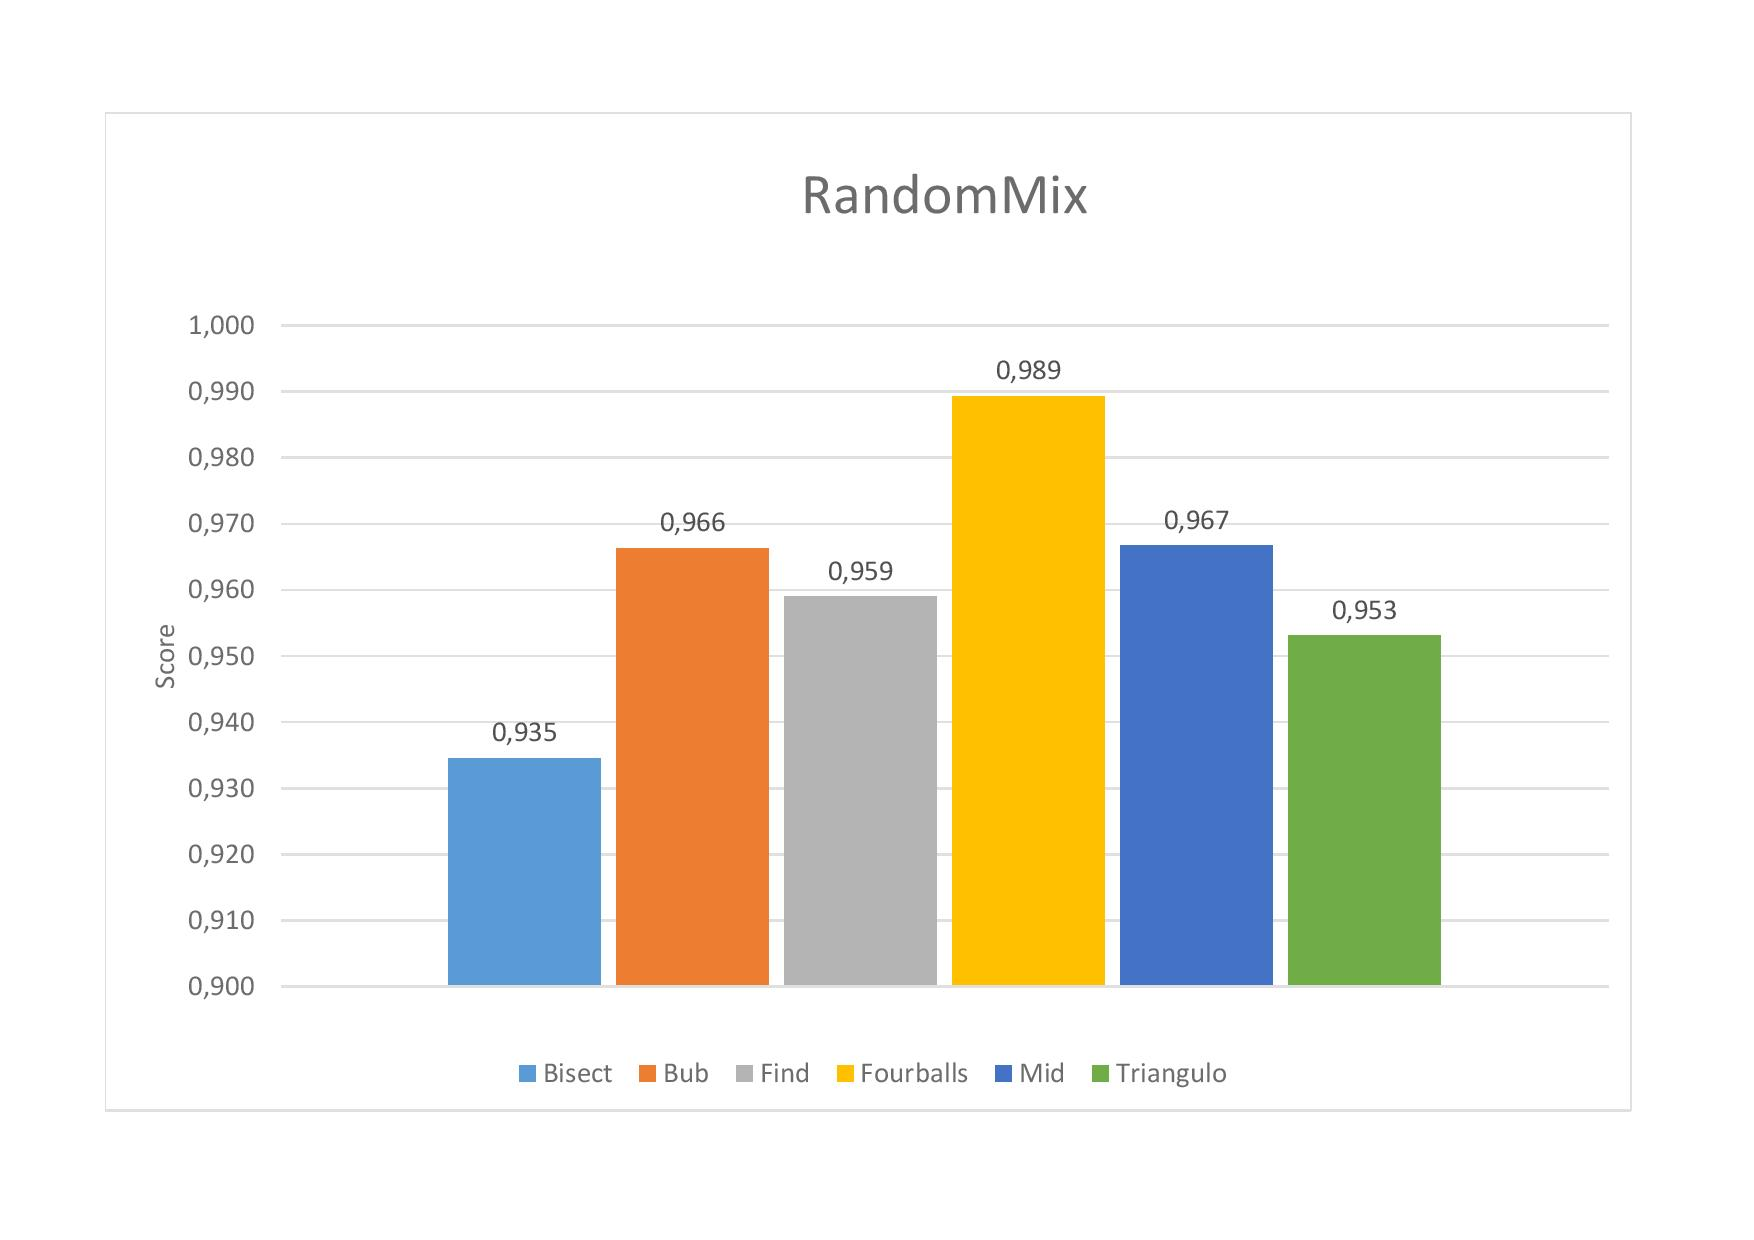
\includegraphics[width=1\textwidth]{graficos/strategies/randommix.jpg}
\caption{\textit{Scores} dos problemas usando a estratégia Random}
\label{fig:Random}
\end{figure}
Com o \textit{score} média média igual a 0.961 e desvio padrão a 0.016, podemos dizer que, no geral, esta estratégia parece ser uma solução razoável comparada às demais SOMs, porém ainda perdendo para as de Mutação seletiva.

\subsubsection{First2Last}
\begin{figure}[H]
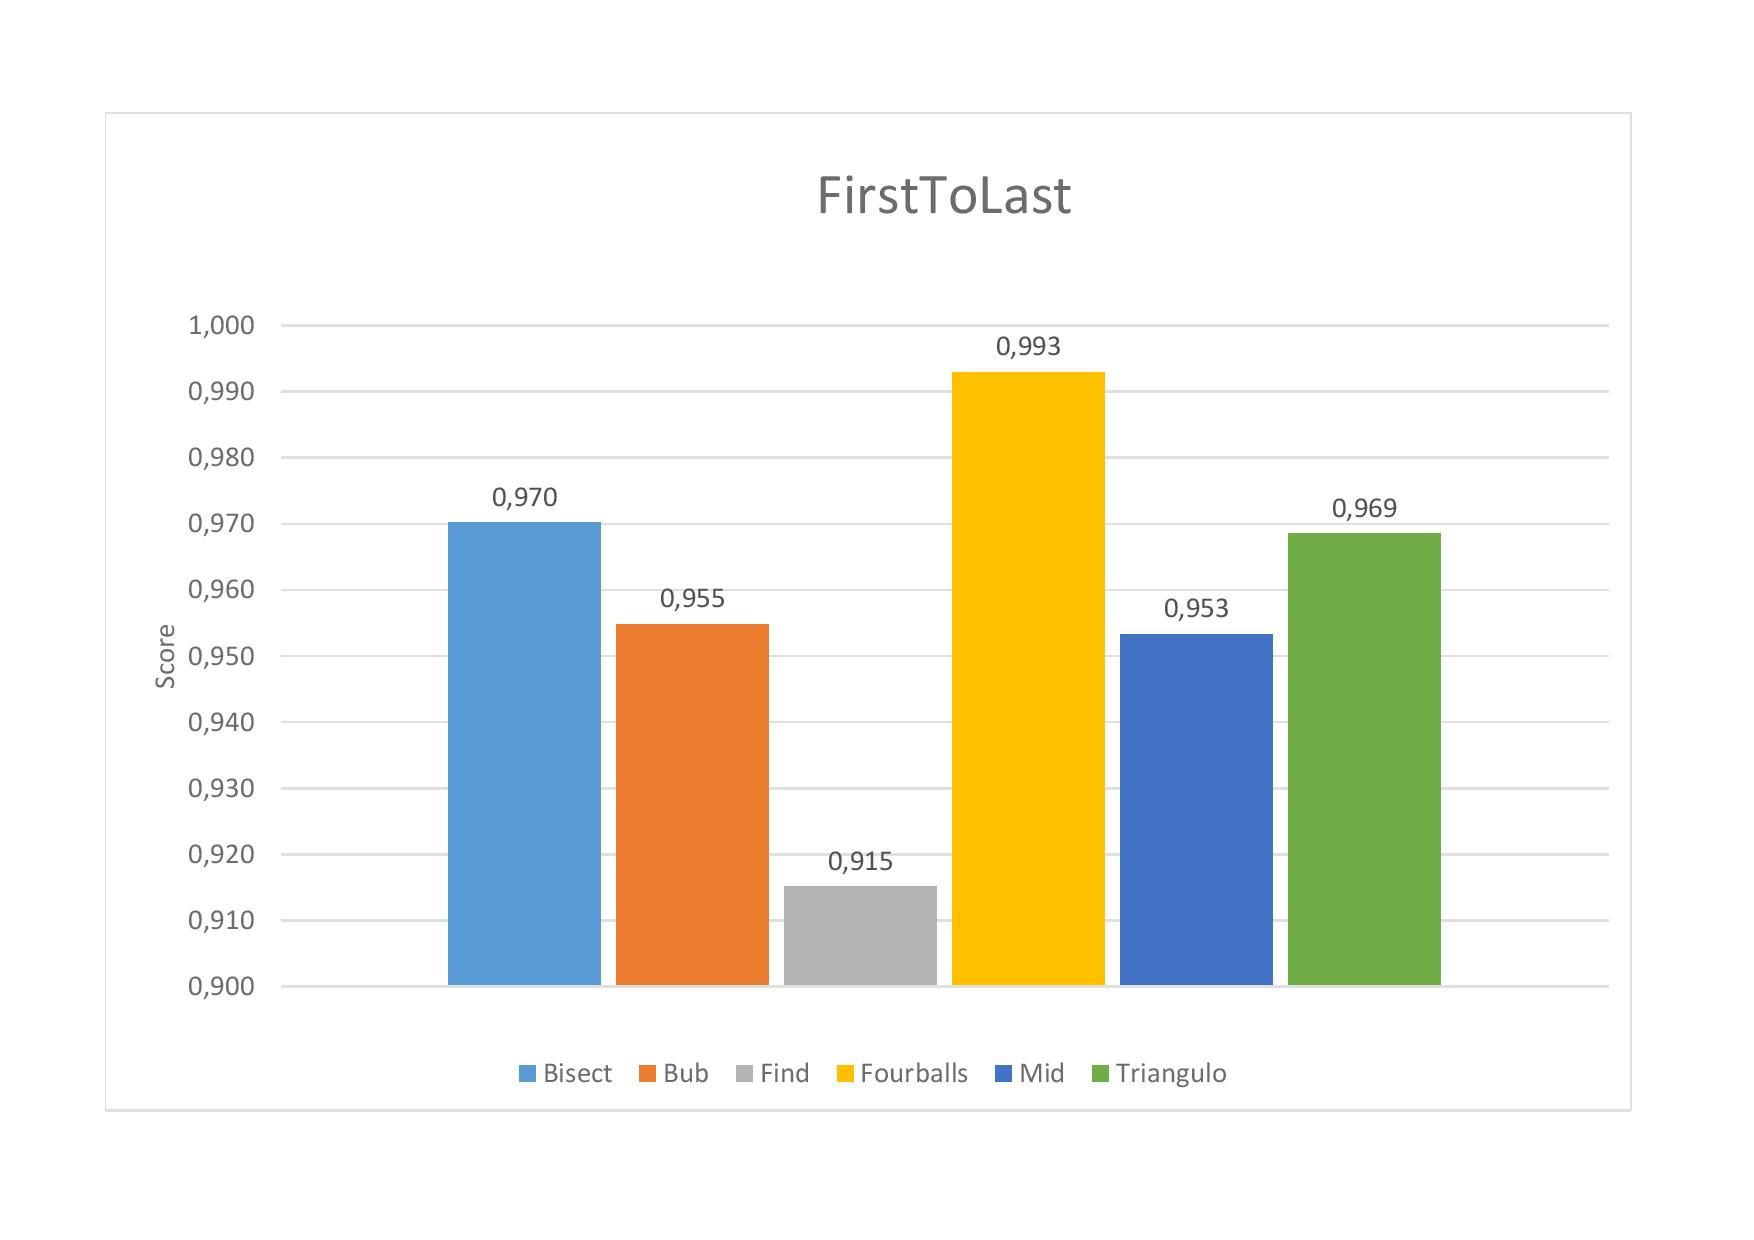
\includegraphics[width=1\textwidth]{graficos/strategies/firsttolast.jpg}
\caption{\textit{Scores} dos problemas usando a estratégia First2Last}
\label{fig:First2Last}
\end{figure}
Já a \textit{First2Last} mostra média menor (0.959) e desvio padrão maior (0.024) quando comparado à \textit{Random}, aparentando ser uma estratégia mais inconstante, no geral.

\subsubsection{Each-choice}
\begin{figure}[H]
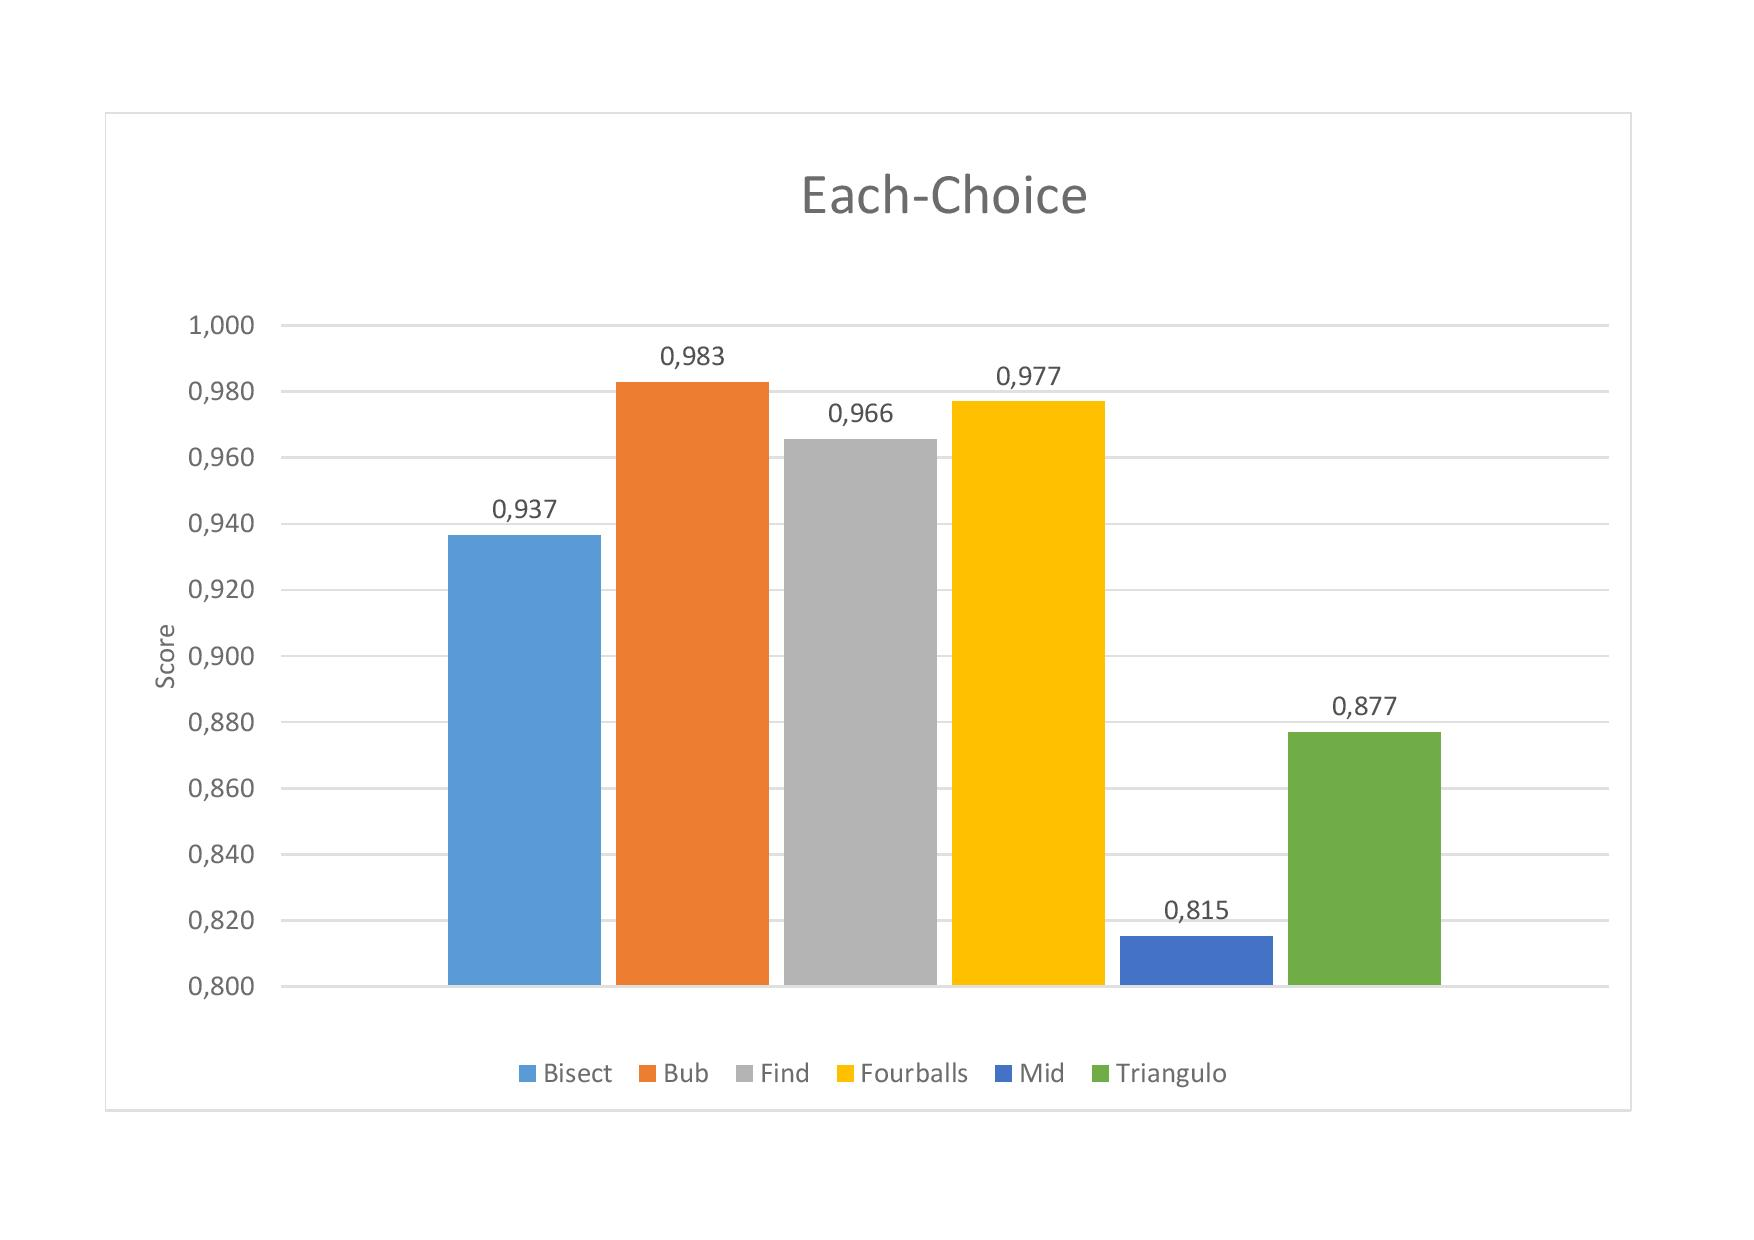
\includegraphics[width=1\textwidth]{graficos/strategies/each-choice.jpg}
\caption{\textit{Scores} dos problemas usando a estratégia Each-choice}
\label{fig:each-choice}
\end{figure}
A \textit{Each-choice} apresenta a maior diferença entre seu máximo e mínimo dentre os SOMs (0.168), a menor média (0.926) e maior desvio padrão, se mostrando ainda mais instável do que a \textit{First2Last}.

\subsubsection{Different-Operators}
\begin{figure}[H]
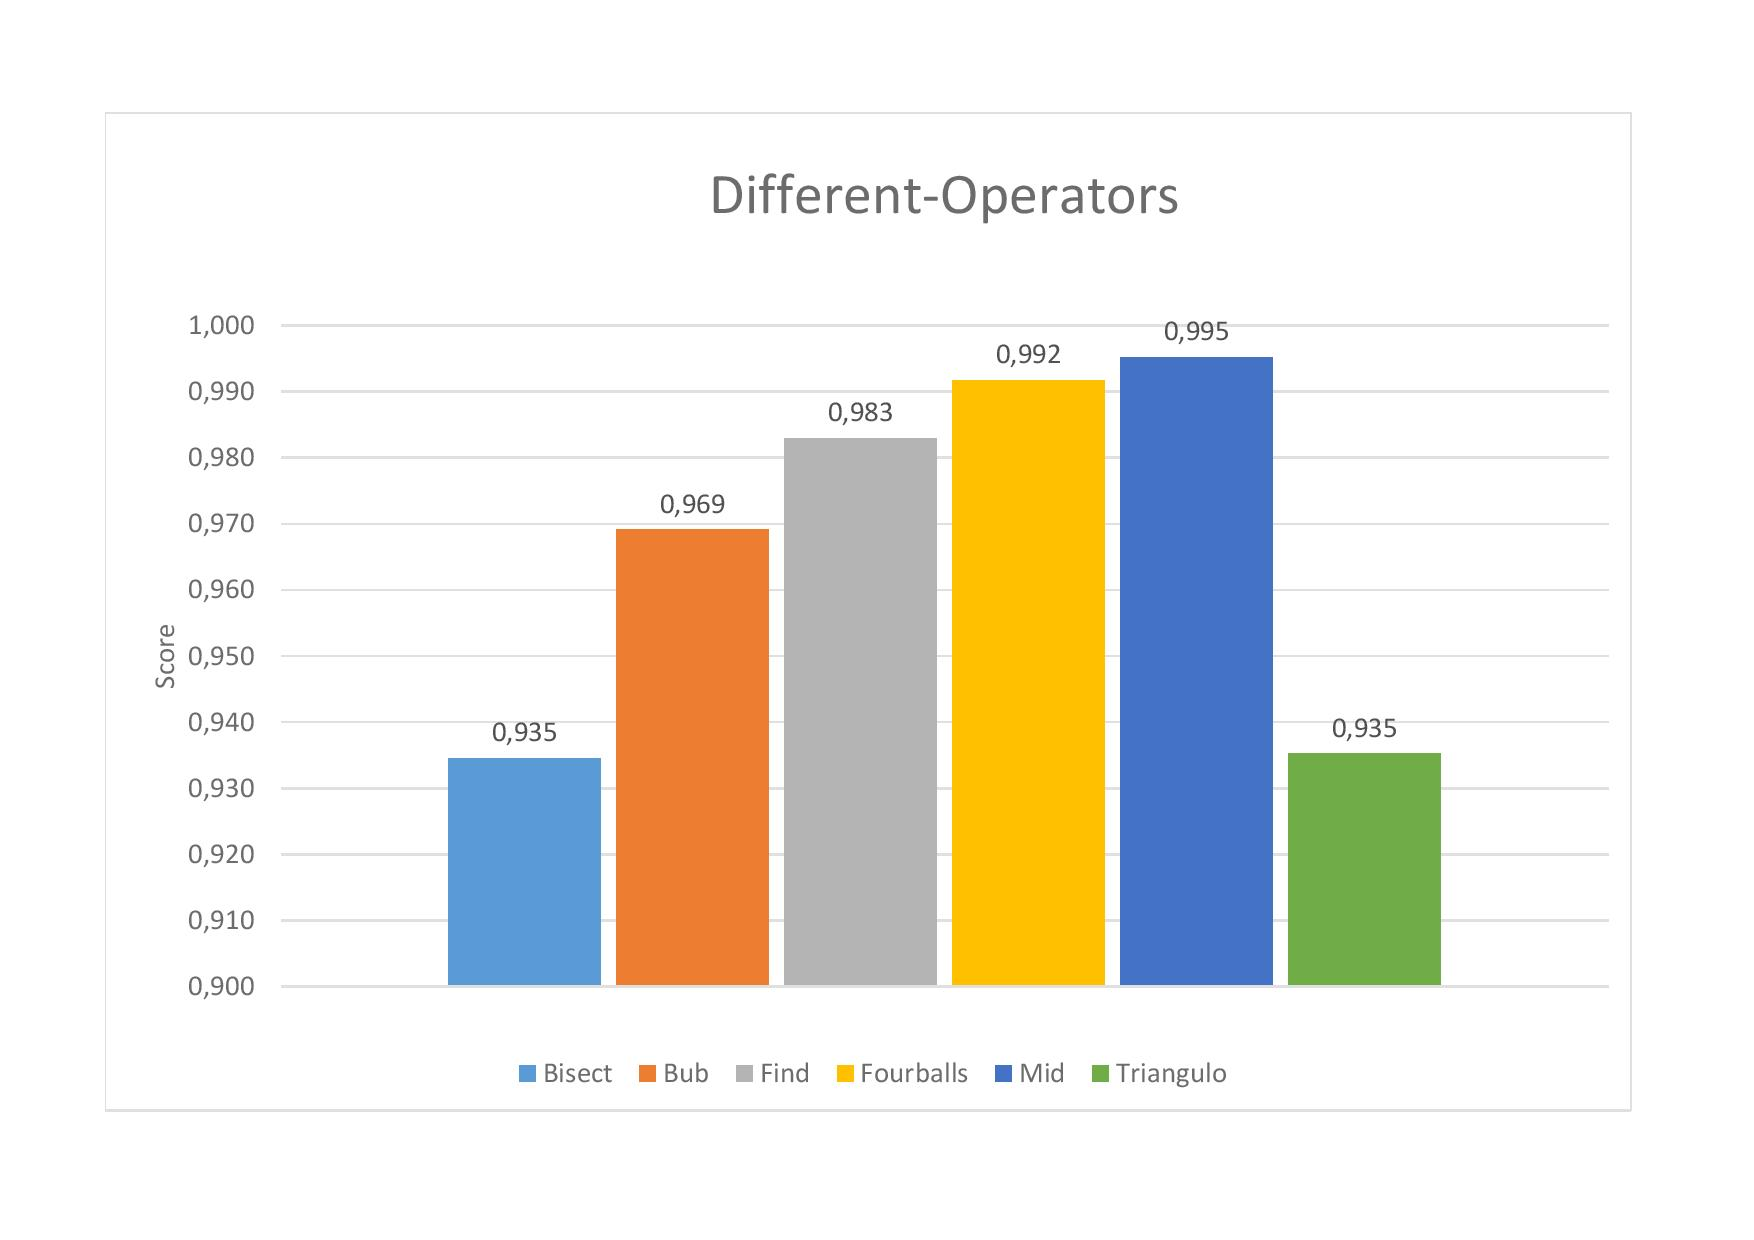
\includegraphics[width=1\textwidth]{graficos/strategies/different-operators.jpg}
\caption{\textit{Scores} dos problemas usando a estratégia Different-operators}
\label{fig:differente-operators}
\end{figure}
A \textit{Different-operators} apresentou a maior média (0.968) entre os SOMs, porém um desvio padrão elevado (0.025), no entando seus 2 maiores \textit{scores} ficaram príxmos de 1.0.

\subsubsection{Mutação seletiva}
\begin{figure}[H]
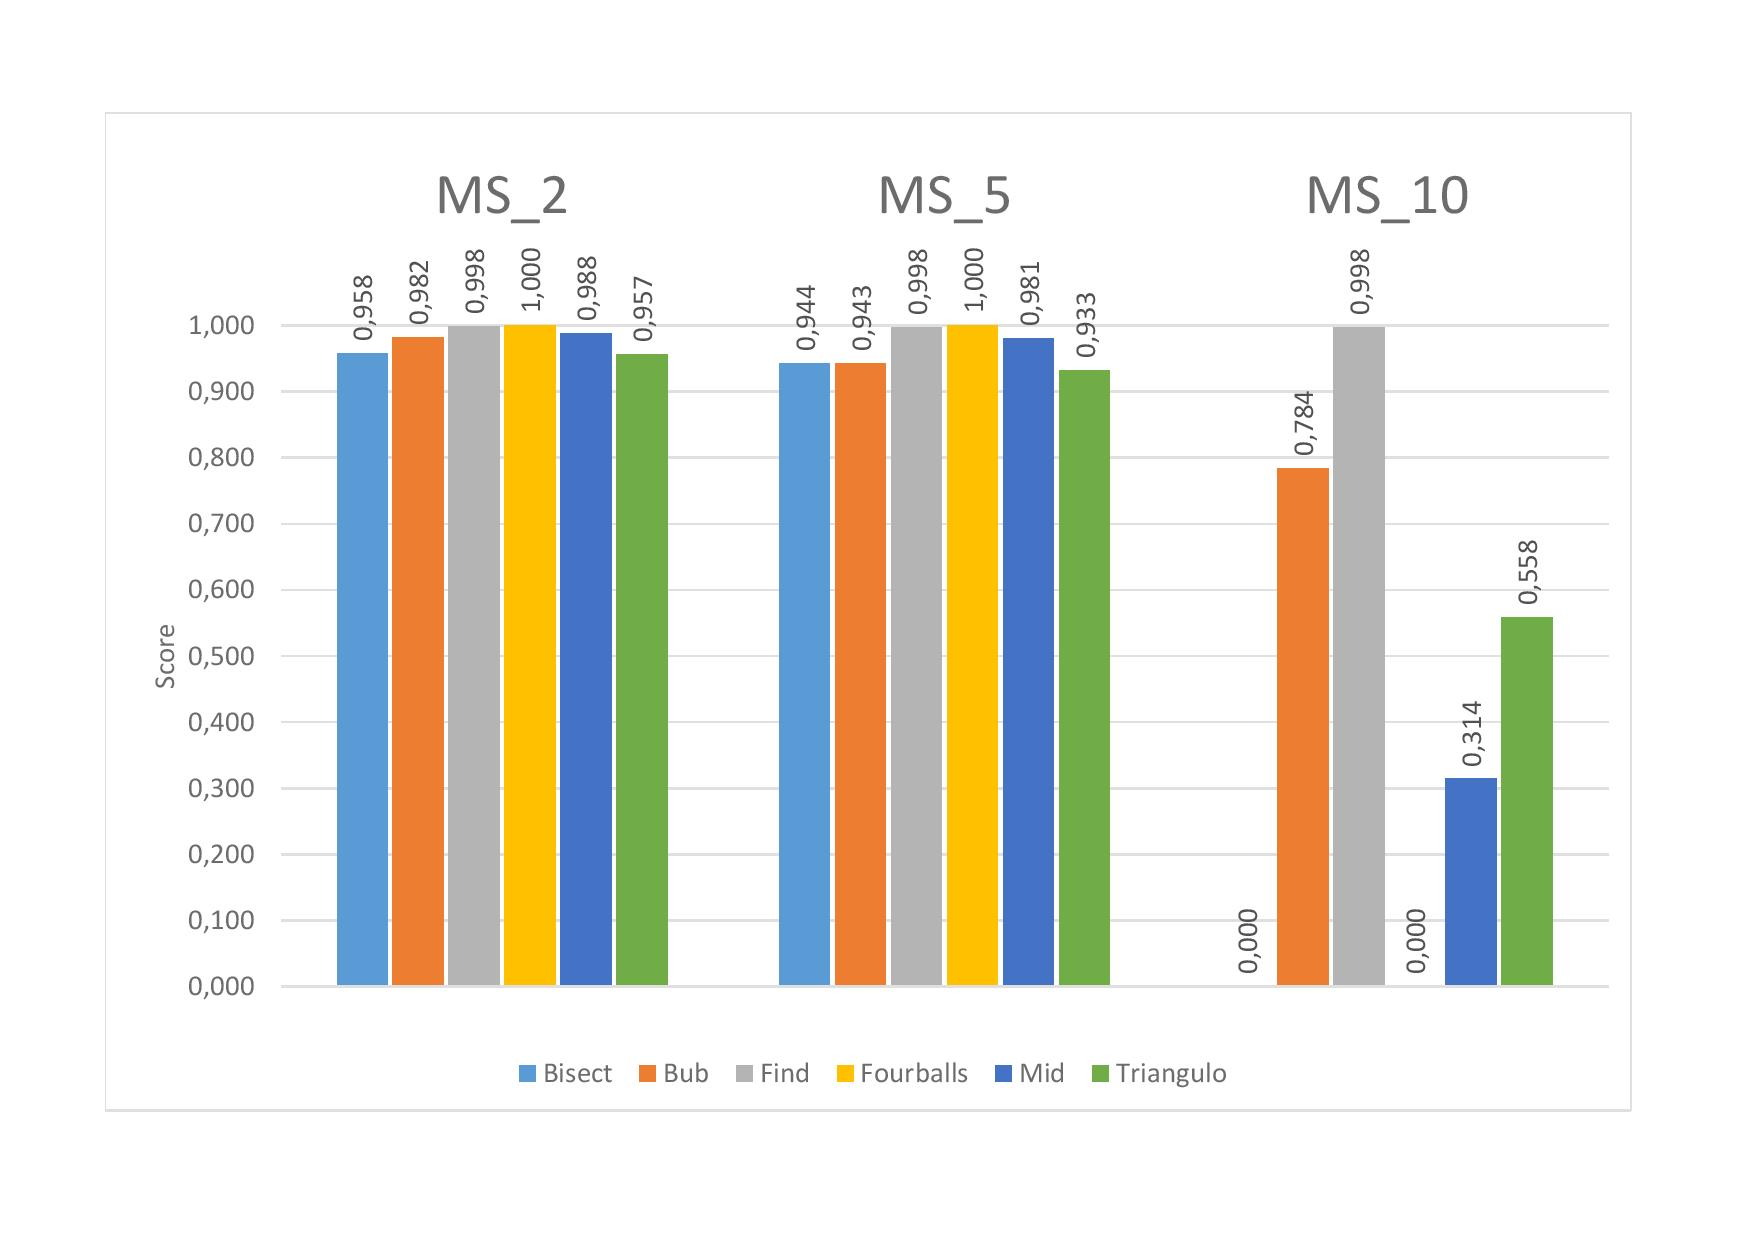
\includegraphics[width=1\textwidth]{graficos/strategies/mss.jpg}
\caption{\textit{Scores} dos problemas usando a estratégia Mutação seletiva}
\label{fig:selective}
\end{figure}
A estratégia MS\_2 apresentou resultados excelentes quando comparado aos SOMs, pois seu \textit{score} mínimo é maior que os dos SOMs e o máximo chegou a 1.0 no problema \textit{Fourballs}. Ainda sim podemos notar que dentre as estratégias de mutação seletiva, ele foi o que se mostrou mais estável com a maior média (0.981) e com desvio padrão igual a 0.017, perdendo por uma diferença menor que 0.001 para o melhor desvio padrão dos SOMs.

A estratégia MS\_5 também mostrou bons resultados, porém com maior variância entre os problemas. Assim como o MS\_2, obteve um \textit{score} máximo e outro muito próximo disso, nos mesmos problemas. Mesmo asism, sua média (0.966) ficou pior que apenas de uma estratégia SOM, a \textit{Different-operators} e com desvio padrão (0.027) maior do que 3 das estratégias SOM.

Já a estratégia MS\_10 se mostrou muito instável, pois em casos de ter poucos operadors na base inicial, restam poucos mutantes para os testes. Em dois dos problemas foram removidos todos os mutantes, porque a base inivial possuía menos de 10 operadores. Mesmo nos problemas onde sobraram mutantes para serem avaliados, seu desempenho ficou muito abaixo do esperado, com uma média de 0.664, a menor entre todas as estratégias avaliadas, e consequentemente o maior desvio padrão (0.255)

\subsubsection{Mutação seletiva - Complemento}
\begin{figure}[H]
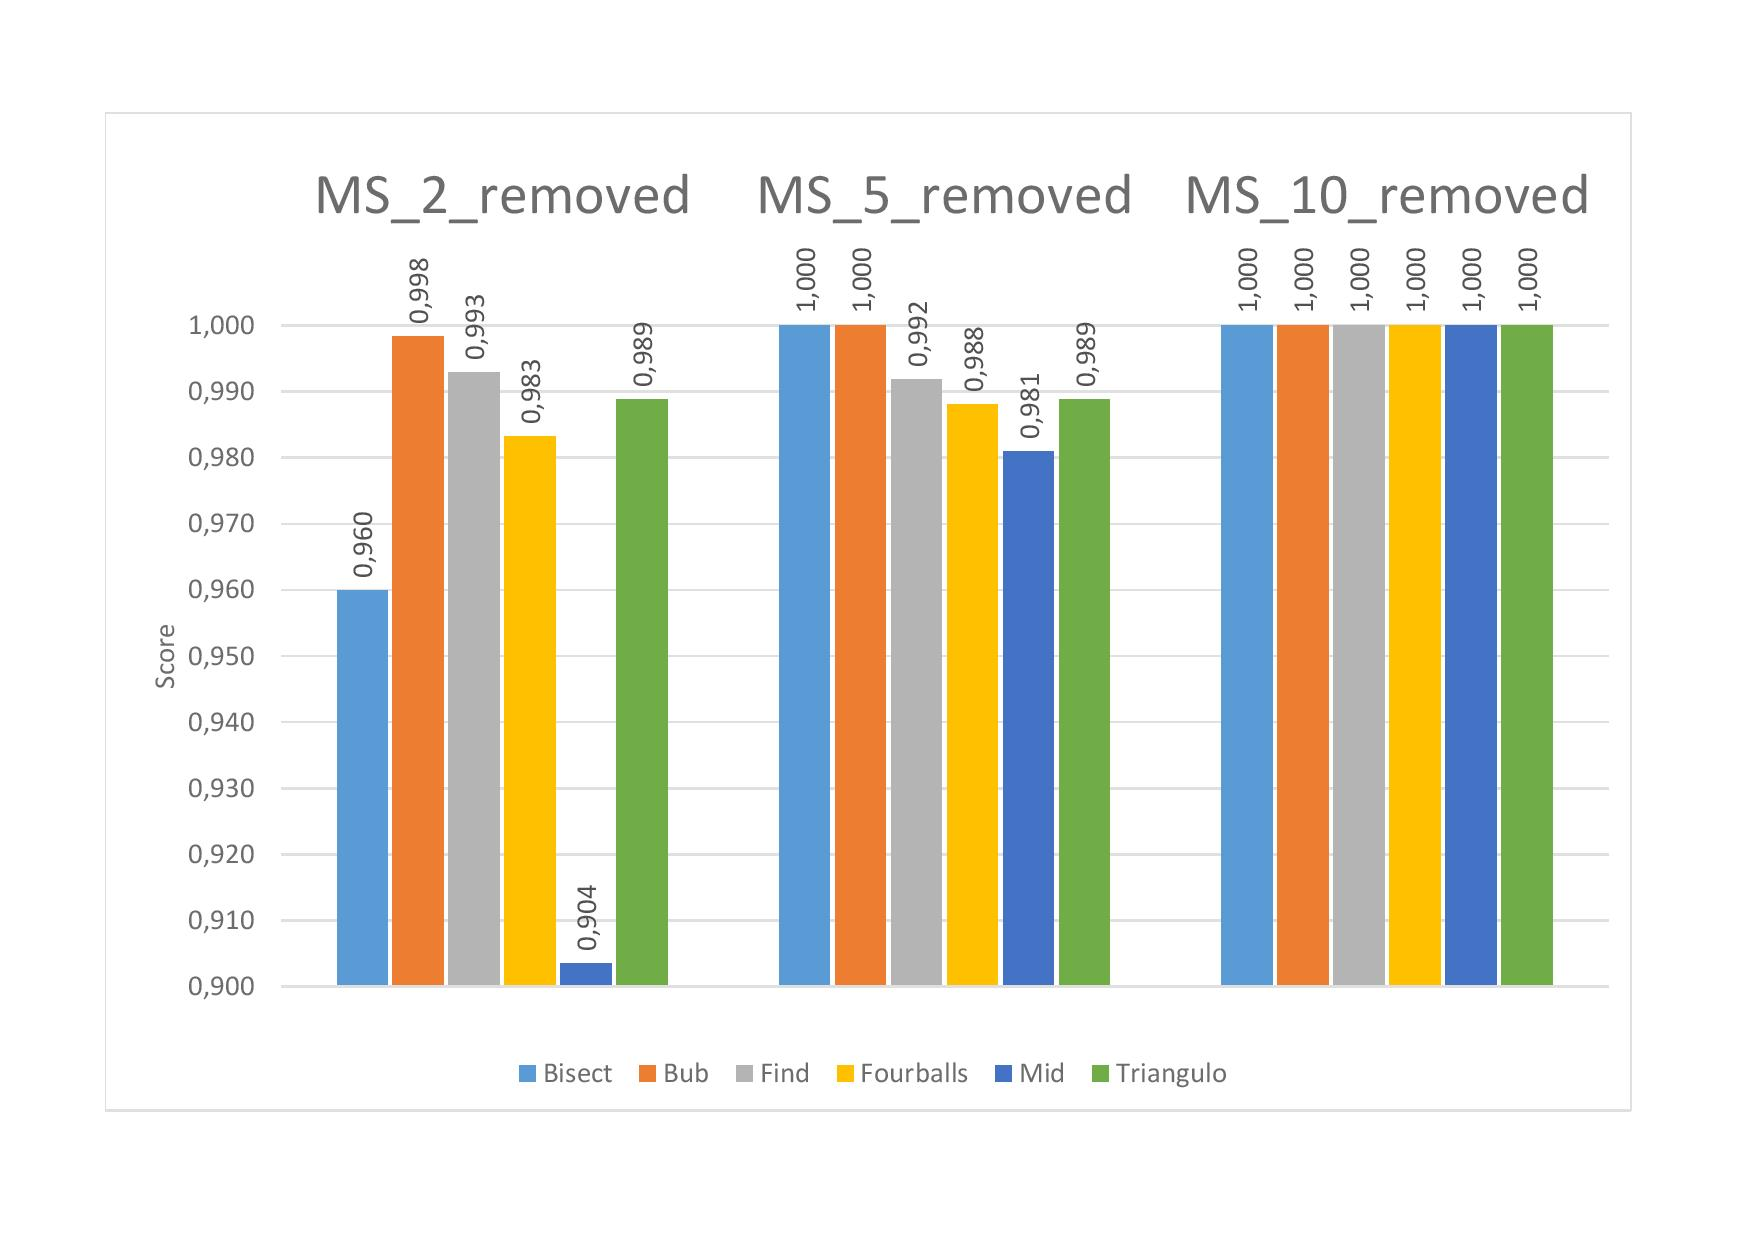
\includegraphics[width=1\textwidth]{graficos/strategies/mss_removed.jpg}
\caption{\textit{Scores} dos problemas usando a estratégia Mutação seletiva - Complemento}
\label{fig:selective-removed}
\end{figure}
As estratégias de mutantes removidos da mutação seletiva (complementares à ela) foram adicionados aos estudos por curiosidade e acabaram se mostrando bons resultados.

A estratégia MS\_2\_removed, mesmo com os mutantes de apenas 2 dos operadores das bases originais, mostrou resultados bons e próximos aos SOMs, com média de 0.971 mas com desvio padrão(0.033) elevado.

Algo surpreendente aconteceu ao ver os resultados da MS\_5\_removed, mesmo sendo apenas uma base complementar, ela se mostrou como a estratégia com \textit{scores} mais estáveis dentre todos os problemas, com média 0.992 e desvio padrão igual a 0.007. Seu \textit{score} mínimo foi de 0.981 (o maior dentre as estratégias apresentadas até agora) e o máximo 1.0. 

A estratégia MS\_10\_removed obteve \textit{scores} perfeitos em todos os problemas, porém em dois deles ele ficou com todos os FOMS e nos outros a maioria deles foi removida, o que acaba na verdade filtrando pouco a base inicial de FOMs, que era o proposto às estratégias.